% Untangling Federal Jurisdiction

% All content comes from Stephen Pratt. I have no idea if he approves of this effort or not.

\documentclass{beamer}
\usetheme{Madrid}
%\usetheme{Goettingen}
\usefonttheme{serif}
\usefonttheme{structuresmallcapsserif}
% \usepackage[font=small,labelfont=bf]{caption}

\setbeamerfont{section title}{parent=title}
\setbeamercolor{section title}{parent=titlelike}
\defbeamertemplate*{section page}{default}[1][]
{
    \centering
    \begin{beamercolorbox}[sep=8pt,center,#1]{section title}
        \usebeamerfont{section title}\insertsection\par
    \end{beamercolorbox}
}
\newcommand*{\sectionpage}{\usebeamertemplate*{section page}}

\makeatletter
\setbeamertemplate{footline}
{
    \leavevmode%
    \hbox{%
    \begin{beamercolorbox}[wd=.333333\paperwidth,ht=2.25ex,dp=1ex,center]{author in head/foot}%
        \usebeamerfont{author in head/foot}\insertshortauthor%~~\beamer@ifempty{\insertshortinstitute}{}{(\insertshortinstitute)}
    \end{beamercolorbox}%
    \begin{beamercolorbox}[wd=.333333\paperwidth,ht=2.25ex,dp=1ex,center]{title in head/foot}%
        \usebeamerfont{title in head/foot}\insertshorttitle
    \end{beamercolorbox}%
    \begin{beamercolorbox}[wd=.333333\paperwidth,ht=2.25ex,dp=1ex,right]{date in head/foot}%
        \usebeamerfont{date in head/foot}\insertshortdate{}\hspace*{2em}
        \insertframenumber{} / \inserttotalframenumber\hspace*{2ex} 
    \end{beamercolorbox}}%
    \vskip0pt%
}
\makeatother

\begin{document}
\title[Untangling Federal Jurisdiction]{Untangling Federal Jurisdiction Within a State}
\author{Stephen Pratt}

\frame{\titlepage}

\begin{frame}{Thomas Paine, 1737-1809}
    \begin{columns}[c]
        \column{2in}
            \begin{figure}[h]
                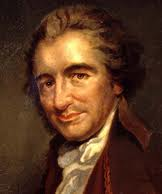
\includegraphics{img/thomas-paine.png}
            \end{figure}
        \column{1.5in}
            "All power exercised over a nation must have some beginning.  It must either be delegated or assumed.  There are no other sources.  All delegated power is trust, and all assumed power is usurpation.  Time does not alter the nature and quality of either."
    \end{columns}
\end{frame}

\begin{frame}{News Release}
    \begin{block}{March 23, 2012}
    SALT LAKE CITY - Today, Utah Governor Gary R. Herbert signed House Bill 148, which demands the federal government make good on the promises made in the 1894 Enabling Act to extinguish title to federal lands in Utah. 
    \end{block}
\end{frame}

\begin{frame}{News Release}
    \begin{block}{April 25, 2012}
    WASHINGTON – Today, Senator Mike Lee responded to comments made yesterday by Interior Secretary Ken Salazar regarding recent Utah state land transfer legislation.
    \end{block}
\end{frame}

\section{A Recurrence to First Principles}

\frame{\sectionpage}

\begin{frame}
    \begin{columns}[onlytextwidth]
        \column{0.5\textwidth}
            \centering
            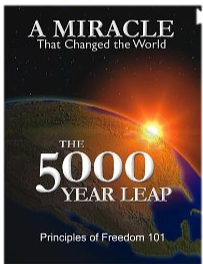
\includegraphics{img/5000-year-leap.png}
            \\ 28
        \column{0.5\textwidth}
        % XXX make this work better
            \pause
            \centering
            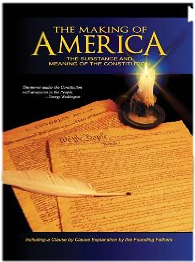
\includegraphics{img/making-of-america.png}
            \\ 286
    \end{columns}
\end{frame}

\begin{frame}{Blackstone's Law Dictionary}
    \begin{columns}[onlytextwidth]
        \column{0.5\textwidth}
            \centering
            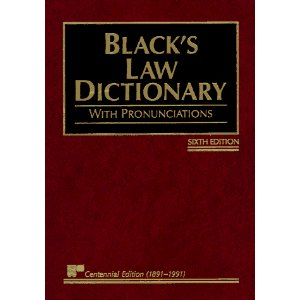
\includegraphics[width=0.75\textwidth]{img/blacks-law.png}
            \\ { \tiny 1920 pages }
        \column{0.5\textwidth}
        \textbf{Jurisdiction} \\
        Page 927 \\
        1.  A government's general power to exercise authority over all persons and things within its territory;
    \end{columns}
\end{frame}

\begin{frame}{Sheriff Gil Gilbertson}
    \begin{columns}[onlytextwidth]
        \column{0.5\textwidth}
            \centering
            Where does the United States Forest Service's authority come from?
            \\ { \tiny October, 2011 }
        \column{0.5\textwidth}
            \centering
            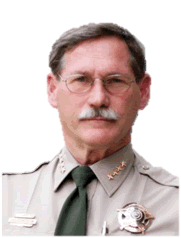
\includegraphics[width=0.75\textwidth]{img/gil-gilbertson.png}
            \\ Sheriff Gil Gilbertson
            \\ Josephine County, Oregon
    \end{columns}
\end{frame}

\begin{frame}{Sheriff Glenn Palmer}
    \begin{columns}[onlytextwidth]
        \column{0.5\textwidth}
            \centering
            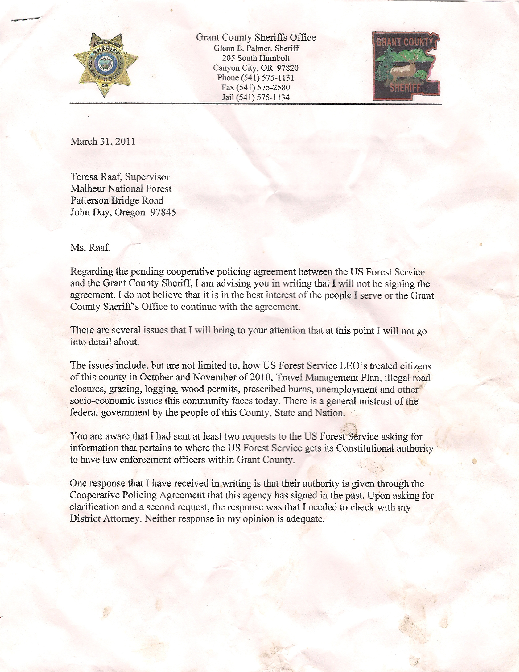
\includegraphics[width=0.75\textwidth]{img/glenn-palmer-letter.png}
            \\ { \tiny March 31, 2011 }
        \column{0.5\textwidth}
            \centering
            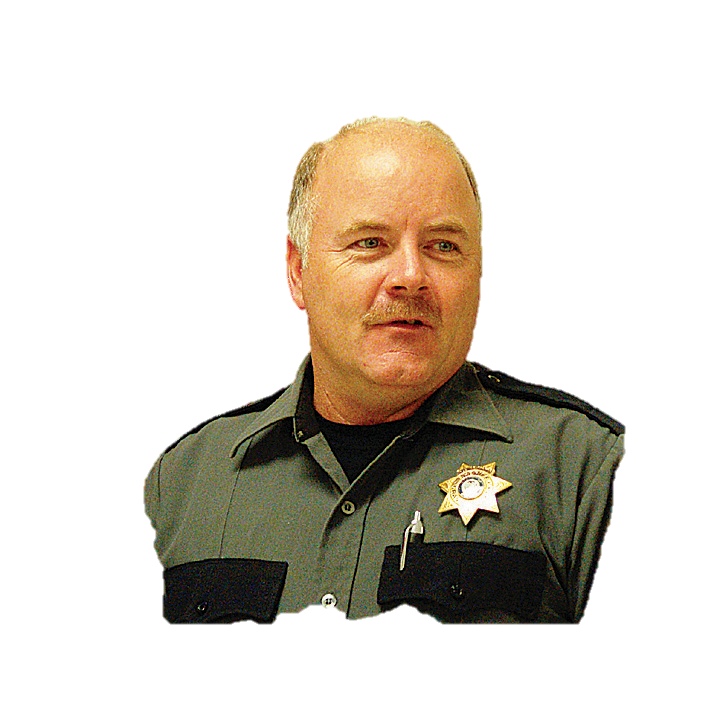
\includegraphics[width=0.75\textwidth]{img/glenn-palmer.png}
            \\ Sheriff Glenn Palmer
            \\ Grant County, Oregon
    \end{columns}
\end{frame}

\begin{frame}{Sheriff Glenn Palmer}
    \begin{columns}[onlytextwidth]
        \column{0.5\textwidth}
            \centering
            Where does the United States Forest Service get its Constitutional authority to have law enforcement officers in Grant County?
        \column{0.5\textwidth}
            \centering
            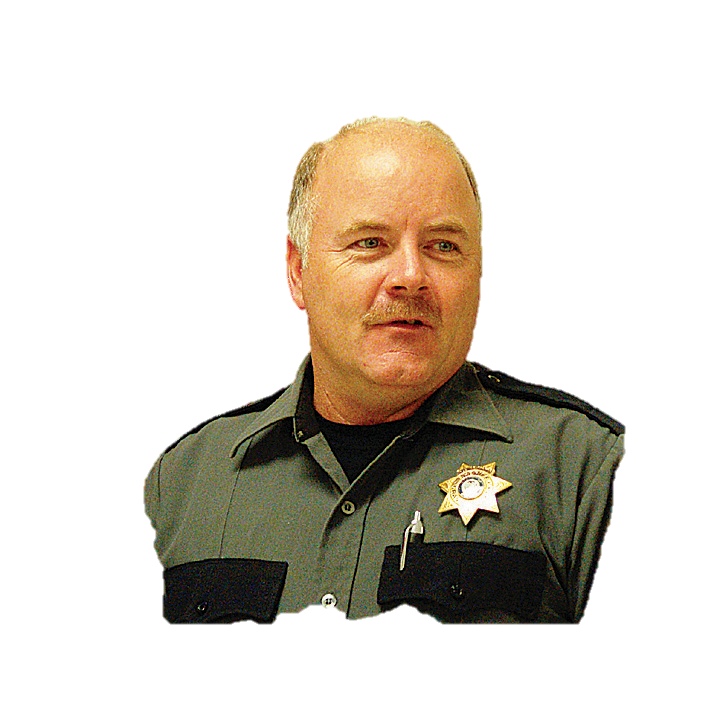
\includegraphics[width=0.75\textwidth]{img/glenn-palmer.png}
            \\ Sheriff Glenn Palmer
            \\ Grant County, Oregon
    \end{columns}
\end{frame}

\begin{frame}{Portland, Oregon}
    
\includegraphics[width=0.3\textwidth]{img/doj.png}
    
\includegraphics[width=0.3\textwidth]{img/usfs.png}
    
\includegraphics[width=0.3\textwidth]{img/ossa.png}
    {   
        \centering
        \\ January 12, 2012 \\
    }
\end{frame}

\begin{frame}{Portland, Oregon}
    \begin{columns}[onlytextwidth]
        \column{0.5\textwidth}
            \centering
            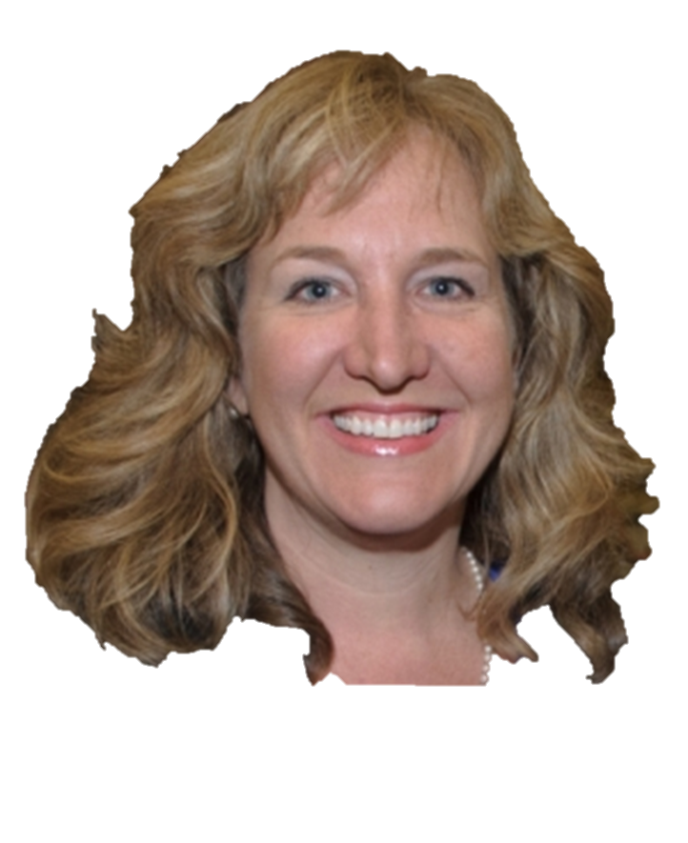
\includegraphics[height=0.28\textheight]{img/amanda-marshall.png}
            \\ United States Attorney \\ S. Amanda Marshall \\
            
\includegraphics[height=0.28\textheight]{img/elmer-dickens.png}
            \\ Washington County Attorney \\ Elmer M. Dickens \\

        \column{0.5\textwidth}
            \centering
            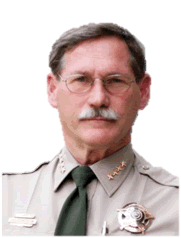
\includegraphics[height=0.28\textheight]{img/gil-gilbertson.png}
            \\ Sheriff Gil Gilbertson \\ Josephine County \\
            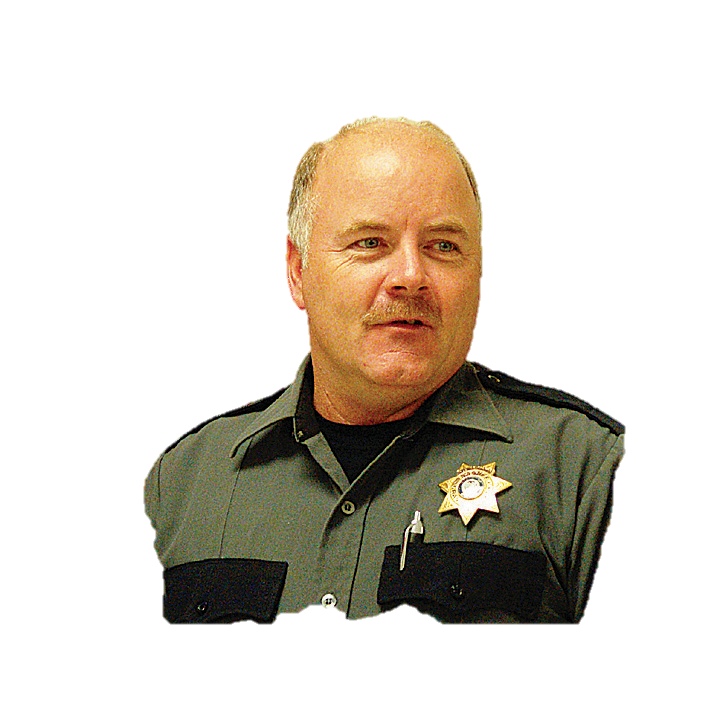
\includegraphics[height=0.28\textheight]{img/glenn-palmer.png}
            \\ Sheriff Glenn Palmer \\ Grant County \\

    \end{columns}
\end{frame}

\begin{frame}
    \begin{columns}[onlytextwidth]
        \column{0.5\textwidth}
What bothered me the most regarding the conversation in Portland with the US
Attorney's office was that they did not want to talk about the Constitution,
but rather put all their confidence in the Supreme Court rulings. They even
referred to the ``Supreme Law of the Land'' as the Supreme Court and were visibly
upset that I would object to that notion
        \column{0.5\textwidth}
            \centering
            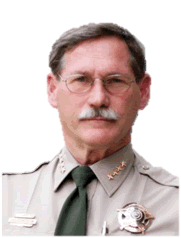
\includegraphics[width=0.75\textwidth]{img/gil-gilbertson.png}
            \\ Sheriff Gil Gilbertson
            \\ (Personal email, February 29, 2012)
    \end{columns}
\end{frame}

\begin{frame}{Summary and Opinion, January 13, 2012}
    \begin{columns}[onlytextwidth]
        \column{0.5\textwidth}
        There are many Supreme Court cases going back over a hundred years\ldots \\
        \vspace{16pt}
        The federal Congress, well over one hundred years ago\ldots
        \column{0.5\textwidth}
            \centering
            
\includegraphics[width=0.75\textwidth]{img/elmer-dickens.png}
            \\ Attorney Elmer Dickens \\
    \end{columns}
\end{frame}

\begin{frame}{Summary and Opinion, January 13, 2012}
    \begin{columns}[onlytextwidth]
        \column{0.5\textwidth}
To put it bluntly, the opinion that federal agents do not have jurisdiction on federal property located within the State of Oregon is without support in the law and is meritless.
        \column{0.5\textwidth}
            \centering
            
\includegraphics[width=0.75\textwidth]{img/elmer-dickens.png}
            \\ Attorney Elmer Dickens \\
    \end{columns}
\end{frame}

\def\braces#1{[#1]}

\begin{frame}{Summary and Opinion, January 13, 2012}
    \begin{columns}[onlytextwidth]
        \column{0.5\textwidth}
            \centering
            
\includegraphics[width=0.75\textwidth]{img/elmer-dickens.png}
            \\ Attorney Elmer Dickens \\
        \column{0.5\textwidth}
\ldots it appears that the sheriff \braces{Gilbertson} does not believe that the US Supreme Court has the authority to interpret the meaning of the US Constitution\ldots
    \end{columns}
\end{frame}

\begin{frame}{Supreme Court, 2012}
    \centering
    {\LARGE How \emph{trustworthy} are the decisions of the Supreme Court? } \\
    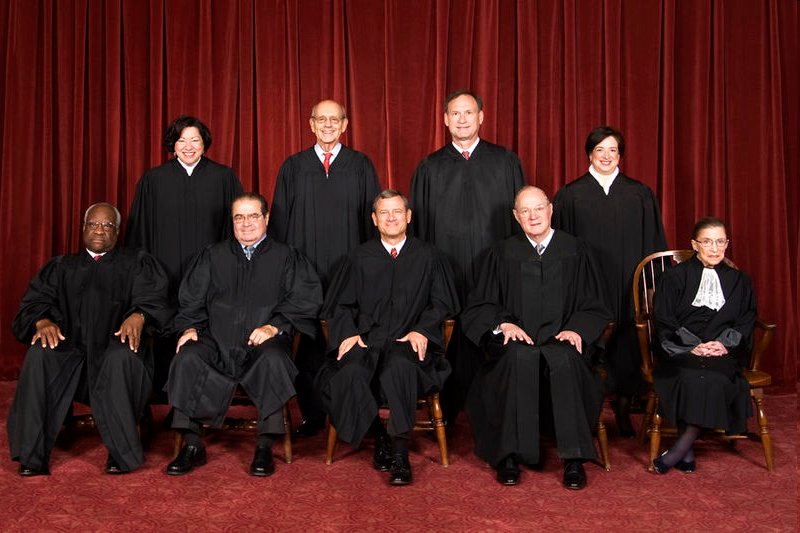
\includegraphics[width=0.9\textwidth]{img/supreme.png} \\
\end{frame}

\begin{frame}{Justice Clarence Thomas}
    \begin{columns}[onlytextwidth]
        \column{0.5\textwidth}
            \centering
            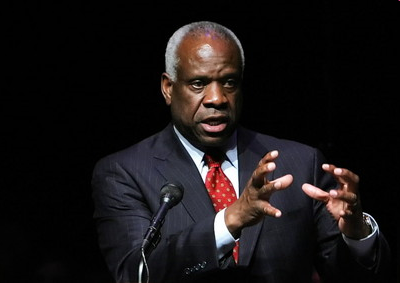
\includegraphics[width=0.75\textwidth]{img/clarence-thomas.png} \\
        \column{0.5\textwidth}
            There are really only two ways to interpret the Constitution: try to discern as best we can what the framers intended or \emph{make it up}.
    \end{columns}
\end{frame}

\begin{frame}{Justice Clarence Thomas}
    \begin{columns}[onlytextwidth]
        \column{0.5\textwidth}
            \centering
            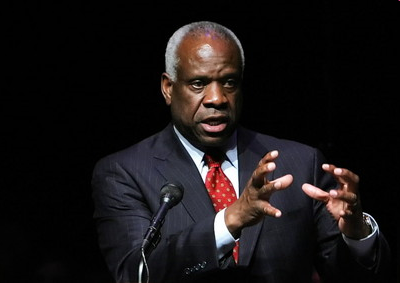
\includegraphics[width=0.75\textwidth]{img/clarence-thomas.png} \\
        \column{0.5\textwidth}
        Unless interpretive methodologies are tied to the original intent of the framers, they have no more basis in the Constitution than the latest football scores.
    \end{columns}
\end{frame}

\begin{frame}{TODO\ldots}
    Insert frame here with Justice Thomas looking at Justice Breyer, and talk about making it up.
\end{frame}

\begin{frame}
    \begin{columns}[onlytextwidth]
        \column{0.5\textwidth}
            \centering
            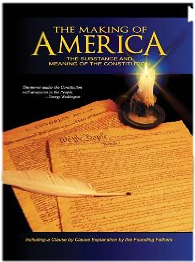
\includegraphics[width=0.75\textwidth]{img/making-of-america.png} \\
            W. Cleon Skousen, Lawyer \\
            1985, 888 pages \\

        \column{0.5\textwidth}
            ``\ldots \braces{the Supreme Court} began reversing previous decisions by the bushel basket.''
    \end{columns}
\end{frame}

\begin{frame}{Usurpation --- Timothy B. Lewis}
    Show a decent shot of Timothy B. Lewis and/or his book \\
    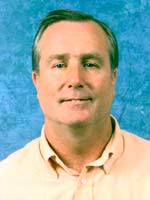
\includegraphics{img/timothy-lewis.png}
\end{frame}

\begin{frame}{The Supremacists --- Phyllis Schlafly}
    \begin{columns}[onlytextwidth]
        \column{0.5\textwidth}
            \centering
            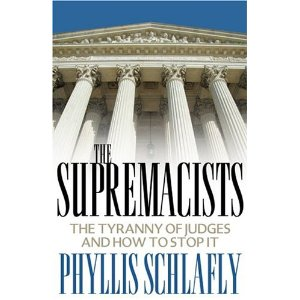
\includegraphics[width=0.75\textwidth]{img/the-supremacists.png} \\
            2004, 246 pages \\

        \column{0.5\textwidth}
            \centering
            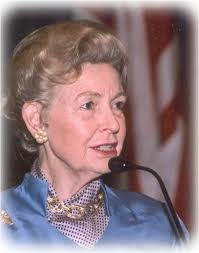
\includegraphics[width=0.75\textwidth]{img/phyllis-schlafly.png} \\
            Lawyer \\
    \end{columns}
\end{frame}

\begin{frame}{Men in Black --- Mark Levin}
    \begin{columns}[onlytextwidth]
        \column{0.5\textwidth}
            \centering
            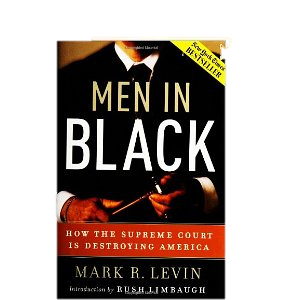
\includegraphics[width=0.75\textwidth]{img/men-in-black.png} \\

        \column{0.5\textwidth}
            \centering
            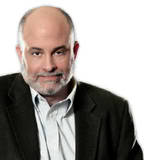
\includegraphics[width=0.75\textwidth]{img/mark-levin.png} \\
            Lawyer \\
    \end{columns}
\end{frame}

\begin{frame}{Betrayed by the Bench --- John A. Stormer}
    \begin{columns}[onlytextwidth]
        \column{0.5\textwidth}
            \centering
            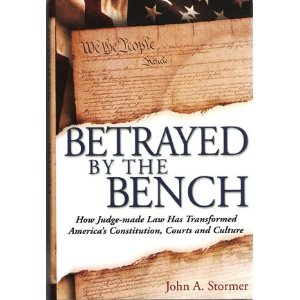
\includegraphics[width=0.75\textwidth]{img/betrayed-by-the-bench.png} \\

        \column{0.5\textwidth}
            \centering
            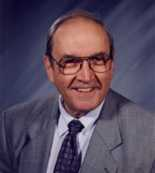
\includegraphics[width=0.75\textwidth]{img/john-stormer.png} \\
            John A. Stormer, \textbf{None Dare Call it Treason} \\
            \emph{(Millions of sales)} \\
    \end{columns}
\end{frame}

\begin{frame}{Constitutional Law for Enlighted Citizens --- Michael Farris}
    \begin{columns}[onlytextwidth]
        \column{0.5\textwidth}
            \centering
            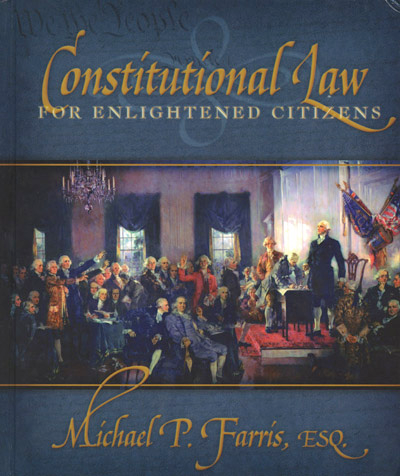
\includegraphics[width=0.75\textwidth]{img/constitutional-law.png} \\
            2006, 579 pages \\

        \column{0.5\textwidth}
            \centering
            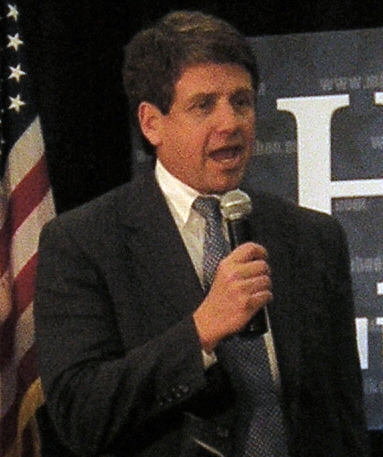
\includegraphics[width=0.75\textwidth]{img/michael-farris.png} \\
            Michael Farris, Lawyer
    \end{columns}
\end{frame}

\begin{frame}{Constitutional Law for Enlighted Citizens --- Michael Farris}
    \begin{columns}[onlytextwidth]
        \column{0.5\textwidth}
            \centering
            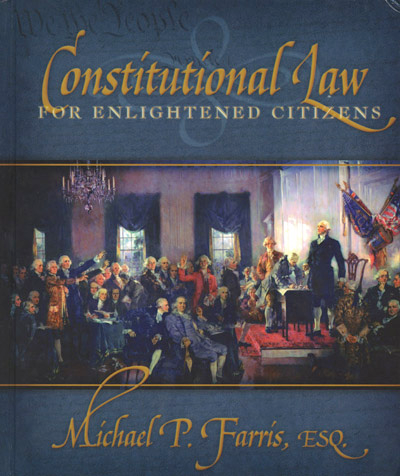
\includegraphics[width=0.75\textwidth]{img/constitutional-law.png} \\
            2006, 579 pages \\

        \column{0.5\textwidth}
            ``The Court has twisted the Constitution and made it an instrument of tyranny\ldots  The Supreme Court makes law out of thin air.'' --- pages 4, 13
    \end{columns}
\end{frame}

\begin{frame}{Constitutional Law for Enlighted Citizens --- Michael Farris}
    \begin{columns}[onlytextwidth]
        \column{0.5\textwidth}
            \centering
            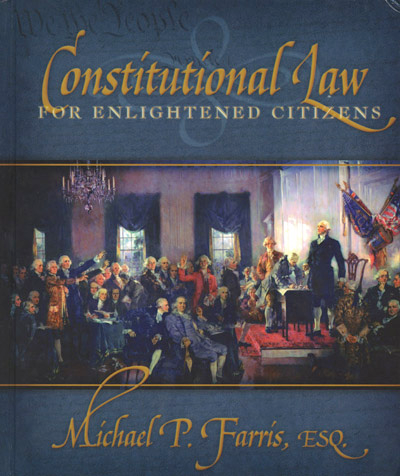
\includegraphics[width=0.75\textwidth]{img/constitutional-law.png} \\
            2006, 579 pages \\

        \column{0.5\textwidth}
            ``All power to make laws shall be vested in Congress. \ldots Today, our freedoms are being stolen from us principally because we have allowed various agencies of government to violate this fundamental principle.'' --- page 8
    \end{columns}
\end{frame}

\begin{frame}{U.S. Attorney S. Amanda Marshall}
    \begin{columns}[onlytextwidth]
        \column{0.5\textwidth}
            \centering
            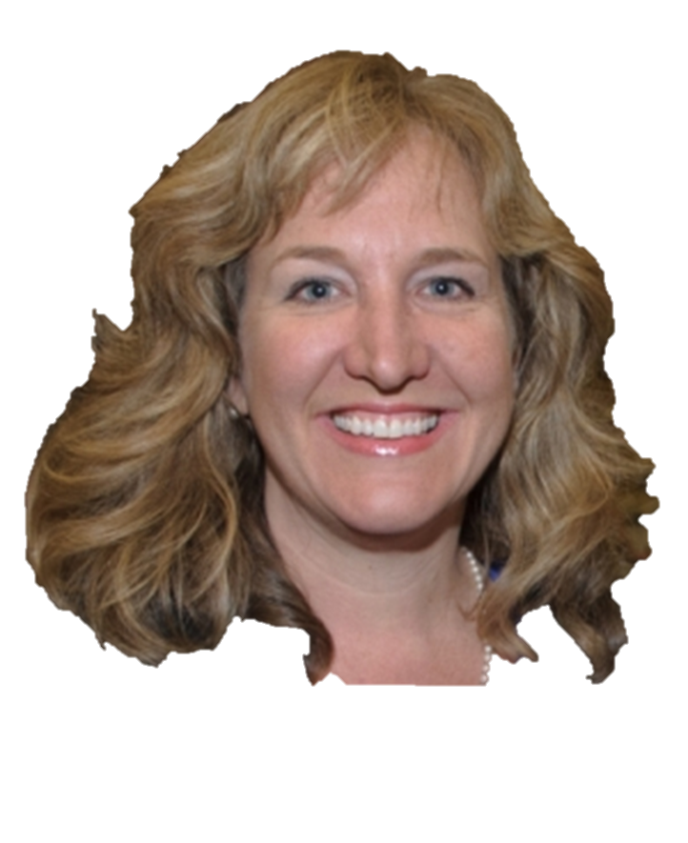
\includegraphics[width=0.75\textwidth]{img/amanda-marshall.png} \\
            United States Attorney S. Amanda Marshall \\

        \column{0.5\textwidth}
            \centering
            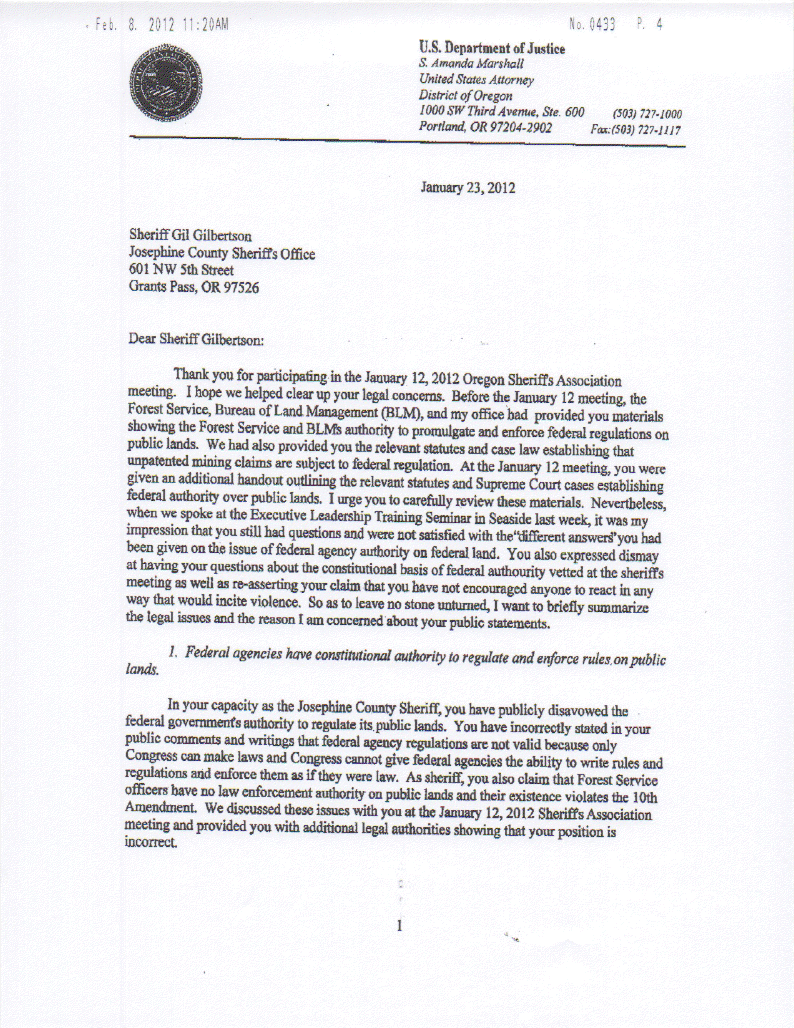
\includegraphics[width=0.75\textwidth]{img/marshall-letter.png} \\
            January 23, 2012 \\
    \end{columns}
\end{frame}

\begin{frame}{U.S. Attorney S. Amanda Marshall}
    \begin{columns}[onlytextwidth]
        \column{0.5\textwidth}
            \centering
            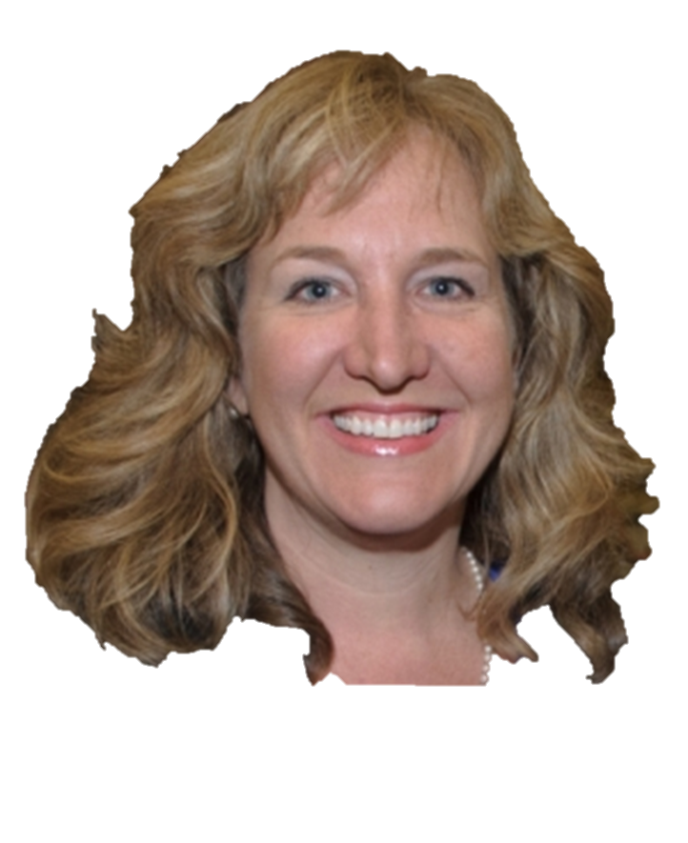
\includegraphics[width=0.75\textwidth]{img/amanda-marshall.png} \\
            United States Attorney S. Amanda Marshall \\

        \column{0.5\textwidth}
            ``Supreme Court precedent for the past one hundred years is clear: under the Property Clause, Congress may delegate rulemaking authority to its federal agencies\ldots''
    \end{columns}
\end{frame}

\begin{frame}{The Supreme Court}
    \centering
    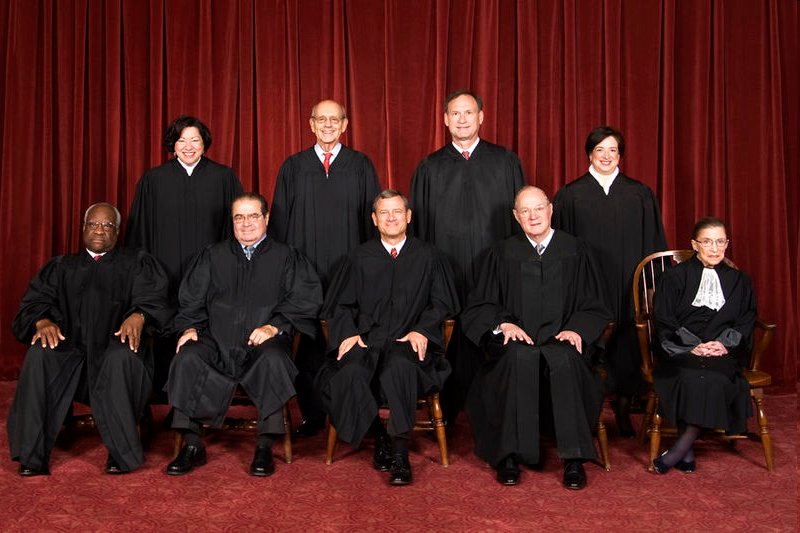
\includegraphics[width=0.75\textwidth]{img/supreme.png} \\
    How trustworty is Supreme Court precendent? How trustworthy is their interpretation of ``the property clause''?
\end{frame}

\begin{frame}{U.S. Attorney S. Amanda Marshall}
    \begin{columns}[onlytextwidth]
        \column{0.5\textwidth}
            \centering
            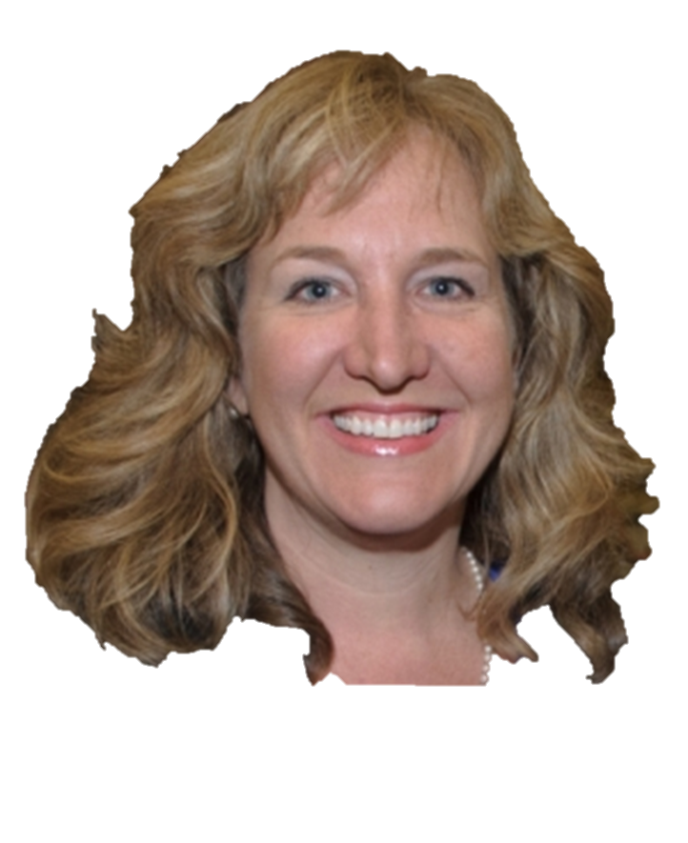
\includegraphics[width=0.75\textwidth]{img/amanda-marshall.png} \\
            United States Attorney S. Amanda Marshall \\

        \column{0.5\textwidth}
            \centering
            ``Your position is incorrect\ldots incorrect\ldots incorrect\ldots \\ erroneous\ldots \braces{You are on a} misguided crusade.'' \\
            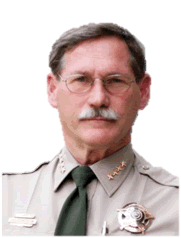
\includegraphics[width=0.3\textwidth]{img/gil-gilbertson.png} \\
    \end{columns}
\end{frame}

\begin{frame}{U.S. Attorney S. Amanda Marshall}
    \begin{columns}[onlytextwidth]
        \column{0.5\textwidth}
            \centering
            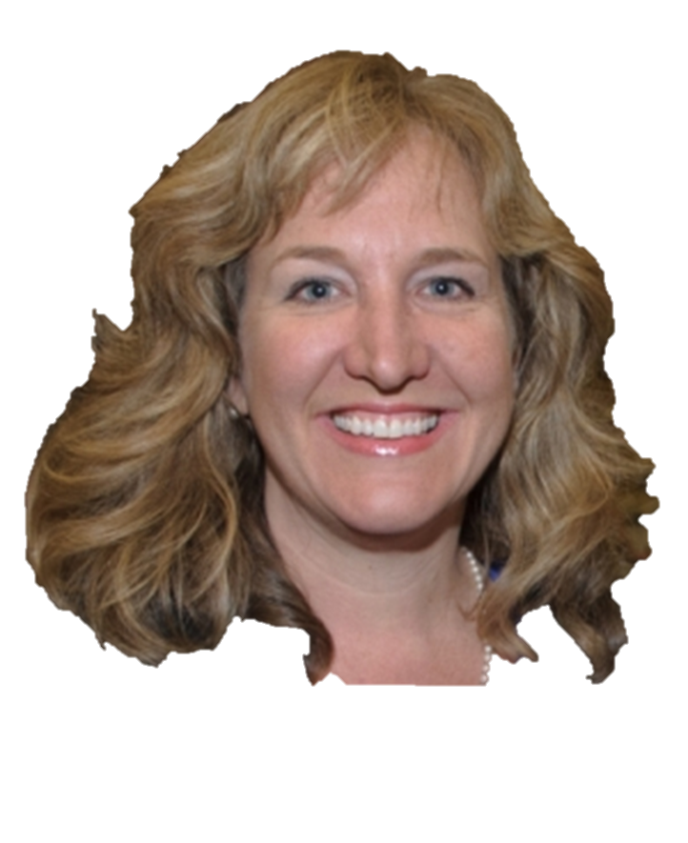
\includegraphics[width=0.75\textwidth]{img/amanda-marshall.png} \\
            United States Attorney S. Amanda Marshall \\

        \column{0.5\textwidth}
            \centering
            ``\braces{It is} your constitutional duty to promote respect for federal laws in your county, particularly when validated by the Supreme Court, whether you agree with them or not.'' \\
            \vspace{10pt}
            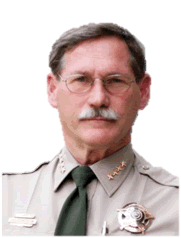
\includegraphics[width=0.3\textwidth]{img/gil-gilbertson.png} \\
    \end{columns}
\end{frame}

\begin{frame}{The Oath?}
    \centering
    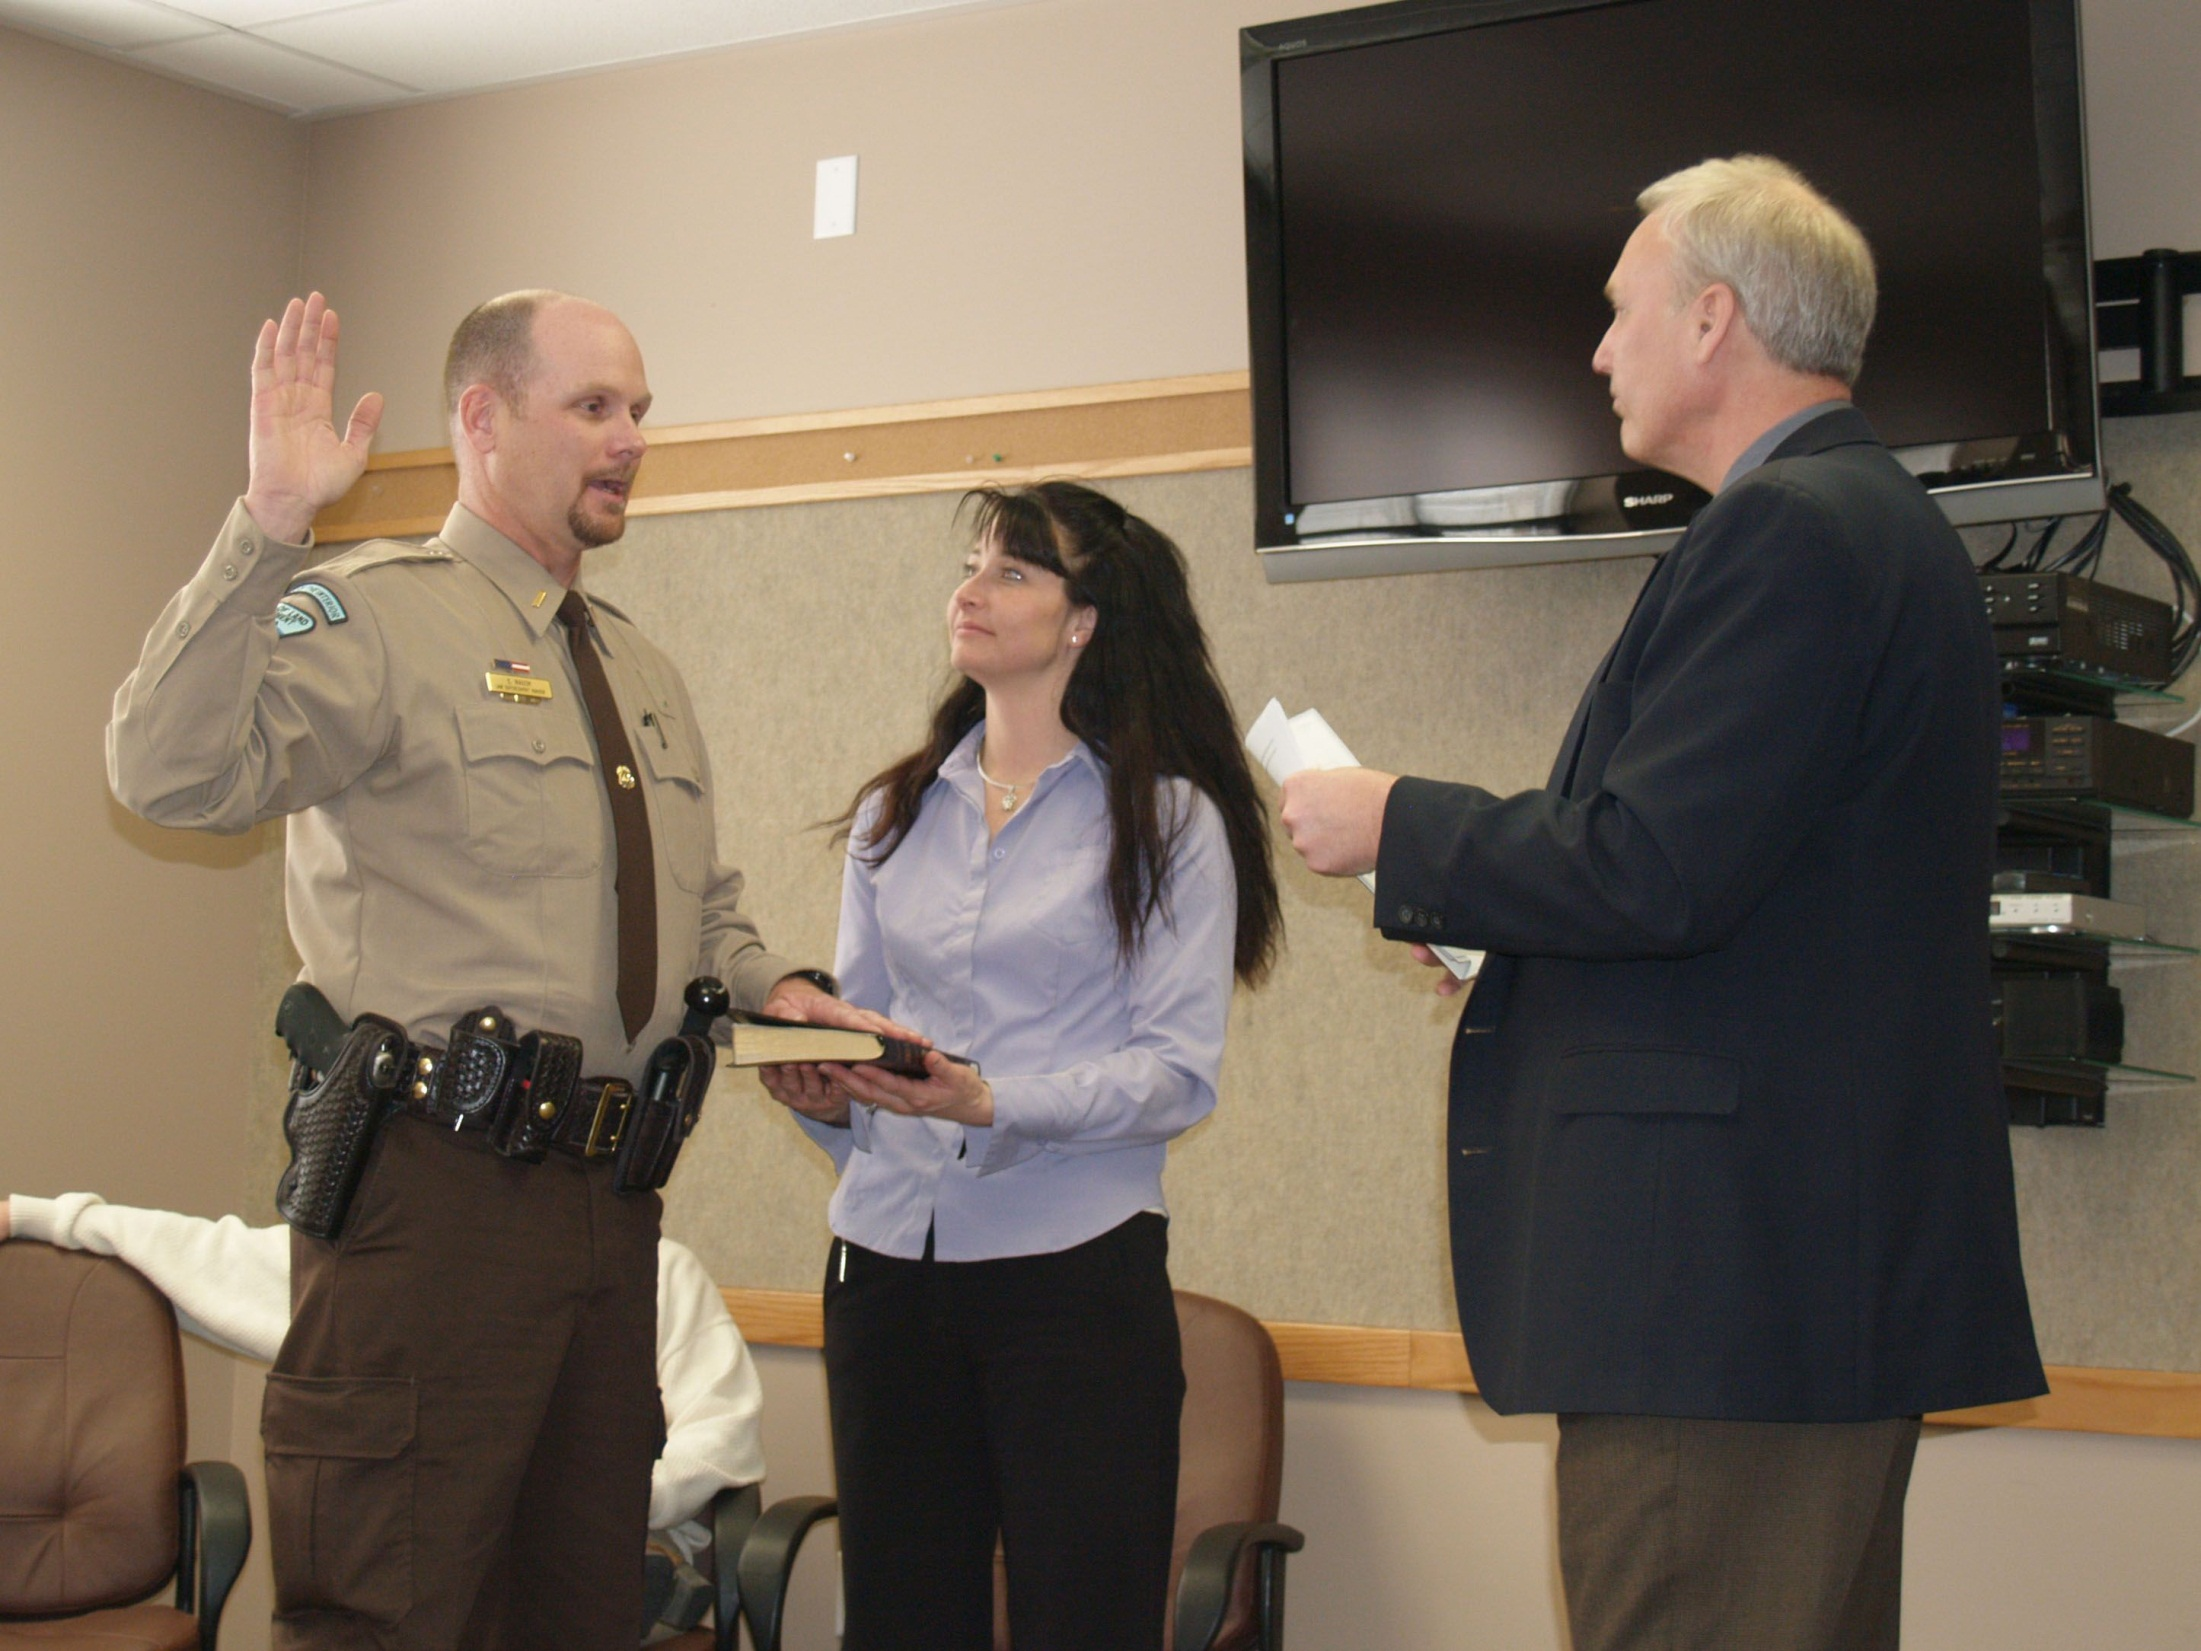
\includegraphics[width=0.7\textwidth]{img/oath.jpg} \\
    I swear to uphold and defend the federal laws and regulations, particularly when validated by the Supreme Court, whether I agree with them or not!
\end{frame}

\begin{frame}{The Oath?}
    \centering
    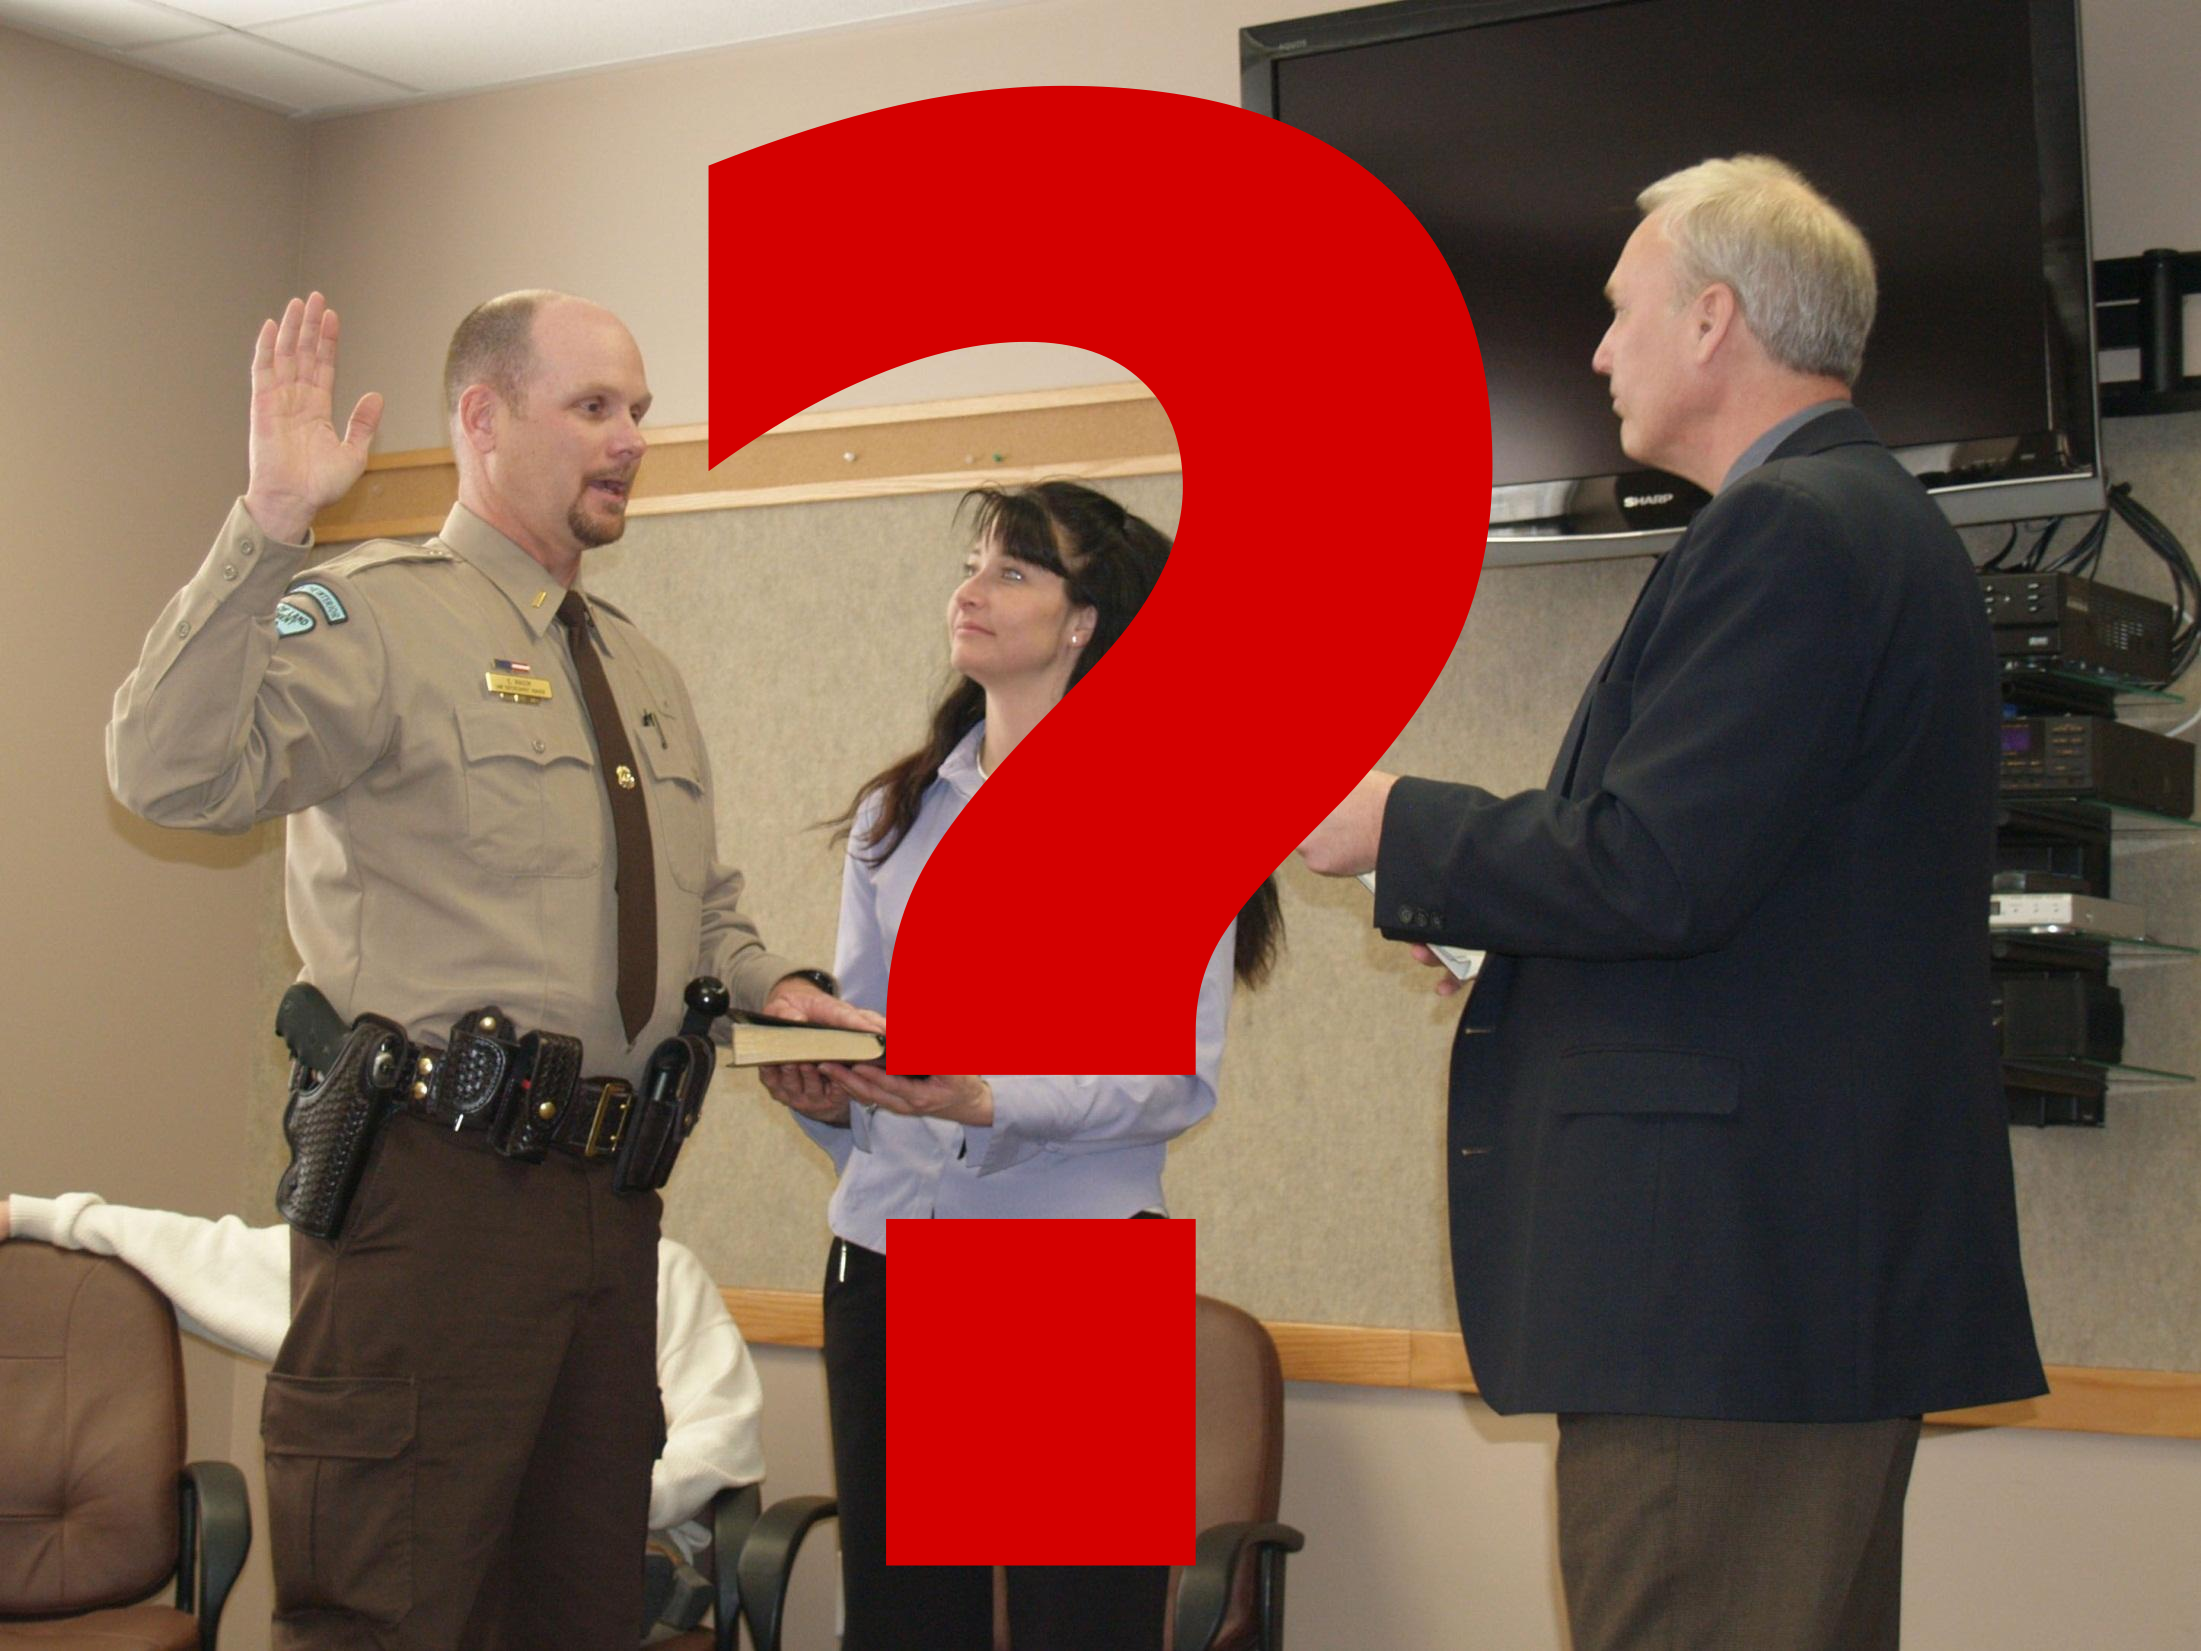
\includegraphics[width=0.7\textwidth]{img/oath-q.png} \\
    I swear to uphold and defend the federal laws and regulations, particularly when validated by the Supreme Court, whether I agree with them or not!
\end{frame}

\begin{frame}{Duty-bound}
    \centering
    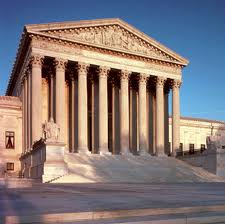
\includegraphics[width=0.3\textwidth]{img/court-bldg.png}
    
\includegraphics[width=0.3\textwidth]{img/sheriff-clip.png}
    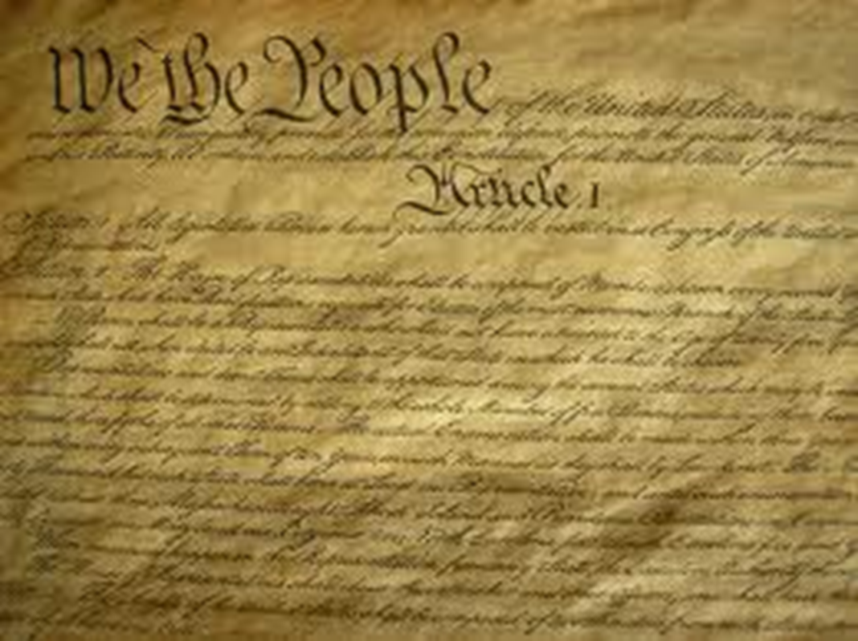
\includegraphics[width=0.3\textwidth]{img/constitution.png} \\
    \vspace{18pt}
    By oath, is a sheriff duty-bound to question the constitutionality of federal laws and court decisions? \\
\end{frame}

\begin{frame}
    \begin{block}{Utah Oath of Office}
    I do solemnly swear (or affirm) that I will support, obey and defend the Constitution of the United States and the Constitution of this State, and that I will discharge the duties of my office with fidelity.
    \end{block}
\end{frame}

\begin{frame}
    \begin{block}{Idaho Oath of Office}
    I do solemnly swear (or affirm, as the case may be) that I will support the Constitution of the United States, and the Constitution of the State of Idaho, and that I will faithfully discharge the duties of (insert office) according to the best of my ability.
    \end{block}
\end{frame}

\begin{frame}
    \begin{block}{U.S. Senate Oath of Office}
    I do solemnly swear (or affirm) that I will support and defend the Constitution of the United States against all enemies, foreign and domestic; that I will bear true faith and allegiance to the same; that I take this obligation freely, without any mental reservation or purpose of evasion; and that I will well and faithfully discharge the duties of the office on which I am about to enter: So help me God.
    \end{block}
\end{frame}

\begin{frame}{Sheriff Cleveland}
    \begin{columns}[onlytextwidth]
        \column{0.5\textwidth}
            \centering
            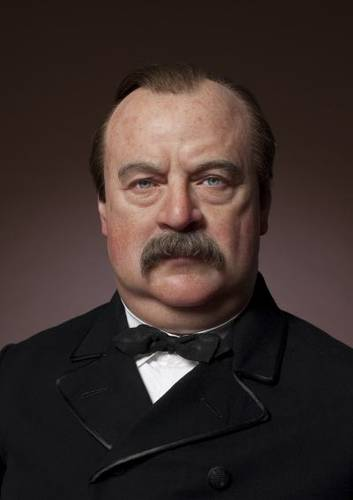
\includegraphics[width=0.75\textwidth]{img/cleveland.png} \\

        \column{0.5\textwidth}
            \centering
            Sheriff Cleveland, 1871 \\
            Erie County, New York
    \end{columns}
\end{frame}

\begin{frame}{How Constitutional are ``Federal Laws''}
    \begin{columns}[onlytextwidth]
        \column{0.5\textwidth}
            \centering
            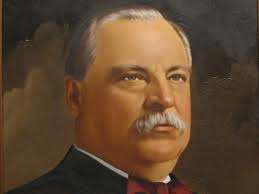
\includegraphics[width=0.75\textwidth]{img/cleveland2.png} \\
            \pause

        \column{0.5\textwidth}
            ``I can find no warrant for such an appropriation in the Constitution.'' \\
            \vspace{15pt}
            Grover Cleveland was faithful to the Founder’s Constitution and to
            what he believed were God’s commandments and common sense.  He
            vetoed 584 Acts of Congress

    \end{columns}
\end{frame}

\begin{frame}{How Constitutional are ``Federal Laws''}
    \begin{columns}[onlytextwidth]
        \column{0.5\textwidth}
            \centering
            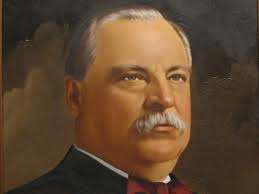
\includegraphics[width=0.75\textwidth]{img/cleveland2.png} \\

        \column{0.5\textwidth}
            ``I ought to have a monument over me when I die, not for anything I have ever done, but for the foolishness I have put a stop to.''

    \end{columns}
\end{frame}

\begin{frame}{How Constitutional are ``Federal Laws''}
    \centering
    { \Huge{The Freedom Index} } \\
    \vspace{10pt}
    \emph{A Congressional Scorecard Based on the U.S. Constitution} \\
    \pause
    January 9, 2012 \\
    \vspace{15pt}
    House / Senate Average Score on Ten Measures: \\
    \vspace{20pt}
    \pause
    \color{red}{\Huge{44\%}} \\
\end{frame}

\begin{frame}{How Constitutional are ``Federal Laws''}
    \centering
    { \Large{United States Senate and House of Representatives }} \\
    \vspace{20pt}
    \includegraphics[width=0.75\textwidth]{img/house-senate-fail.png} \\
\end{frame}

\end{document}
